\begin{pastexam}[label={px:df3-097-ds-02}]{地方三等資訊處理 97 年 第二題}
（申論；20 分）

典型的跳棋棋盤如下圖：
\begin{center}
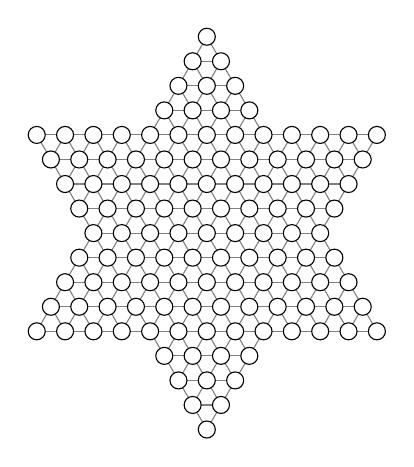
\begin{tikzpicture}[x=3.6mm,y=3.6mm]
\def\ccok#1#2{\pgfmathtruncatemacro{\ccs}{-(#1)-(#2)}%
  \pgfmathtruncatemacro{\ccres}{or(max(#1,#2,\ccs)<=4,min(#1,#2,\ccs)>=-4)}}
\foreach \q in {-8,...,8}{\foreach \r in {-8,...,8}{%
  \ccok{\q}{\r}%
  \ifnum\ccres=1
    \pgfmathtruncatemacro{\qa}{\q+1}\pgfmathtruncatemacro{\ra}{\r+1}\pgfmathtruncatemacro{\qb}{\q-1}%
    \ccok{\qa}{\r}\ifnum\ccres=1 \draw[gray] ({\q+\r/2},{-\r*0.866}) -- ++(1,0);\fi
    \ccok{\q}{\ra}\ifnum\ccres=1 \draw[gray] ({\q+\r/2},{-\r*0.866}) -- ++(0.5,-0.866);\fi
    \ccok{\qb}{\ra}\ifnum\ccres=1 \draw[gray] ({\q+\r/2},{-\r*0.866}) -- ++(-0.5,-0.866);\fi
  \fi}}
\foreach \q in {-8,...,8}{\foreach \r in {-8,...,8}{%
  \ccok{\q}{\r}%
  \ifnum\ccres=1 \filldraw[fill=white,draw=black,thin] ({\q+\r/2},{-\r*0.866}) circle (0.3);\fi}}
\end{tikzpicture}
\end{center}
其中每個圓圈上可放上一顆棋子（紅、黃或綠色）或者不放棋子。現在我們不管跳棋的規則為何或棋子的擺放是否
合理，請你設計一個資料結構來表示任何一種可能的盤面。你必須說明需占用多少空間及如何記錄棋子所在的
位置。（20 分）
\end{pastexam}

\begin{pastsoln}
這是陣列表示法的設計題（資結書第~4.1~節）：重點是把不規則形狀的格子對應到連續的陣列下標，並算出
空間。

\textbf{先數格子}。 棋盤是兩個大三角形疊成的六角星，由上到下 $17$ 列，每列的圓圈數是
\[
1, 2, 3, 4, 13, 12, 11, 10, 9, 10, 11, 12, 13, 4, 3, 2, 1,
\]
合計 $2(1 + 2 + 3 + 4) + 2(13 + 12 + 11 + 10) + 9 = 20 + 92 + 9 = 121$ 個。 每一列都左右對稱，以中線
對齊。

\textbf{每格的狀態}。 每個圓圈有 $4$ 種狀態：空、紅、黃、綠，編成 $0, 1, 2, 3$，剛好用 $2$ 個位元。
題目說不管擺放合不合理，所以每一格的 $4$ 種狀態可以任意組合，可能的盤面共 $4^{121}$ 種；要區分
這麼多種盤面至少需要 $\lg 4^{121} = 242$ 個位元。 下面的設計正好每格 $2$ 位元，已經是最省的。

\textbf{設計：依列編號的一維陣列}。
\begin{enumerate}[label=(\arabic*)]
\item 把 $121$ 個圓圈由上到下、同一列由左到右編號 $0, 1, \ldots, 120$。 盤面就是一個長度 $121$ 的陣列
$\mathit{board}[0..120]$，$\mathit{board}[p]$ 是第 $p$ 號圓圈的狀態（$0$ 空、$1$ 紅、$2$ 黃、$3$ 綠）。
\item 位置用（列 $r$，列內第 $c$ 個）表示，$0 \le r \le 16$，$0 \le c < \mathit{len}[r]$。 另外存兩個
固定的小表：$\mathit{len}[r]$ 是第 $r$ 列的圓圈數（上面那串數字），$\mathit{start}[r]$ 是第 $r$ 列第一個
圓圈的編號（$\mathit{len}$ 的前綴和：$0, 1, 3, 6, 10, 23, 35, 46, 56, 65, 75, 86, 98, 111, 115, 118, 120$）。
位置換成下標：
\[
p = \mathit{start}[r] + c .
\]
例如中間那一列（$r = 8$，$9$ 個）的正中央 $c = 4$，$p = 56 + 4 = 60$。
\item 要畫出盤面或判斷相鄰（跳棋要用），再算每個圓圈的水平座標：以半格為單位，
$x = 2c - (\mathit{len}[r] - 1)$，中線是 $x = 0$。 兩個圓圈相鄰，當且僅當同一列且 $x$ 差 $2$，或上下相鄰
兩列且 $x$ 差 $1$。
\end{enumerate}
\textbf{空間}：
\begin{itemize}
\item 每格 $2$ 位元緊密存放：$121 \times 2 = 242$ 位元，用 $31$ 個位元組（$248$ 位元）存得下。 第 $p$ 格
在第 $\lfloor 2p / 8 \rfloor = \lfloor p/4 \rfloor$ 個位元組的第 $2(p \bmod 4)$、$2(p \bmod 4) + 1$ 個位元，
用位移和遮罩讀寫。
\item 若不在乎省這點空間，用 \texttt{char board[121]} 每格一個位元組，共 $121$ 位元組，存取最簡單。
\item 兩個固定表 $\mathit{len}$、$\mathit{start}$ 各 $17$ 個小整數，和盤面無關，所有盤面共用。
\end{itemize}

\textbf{另一種設計：斜座標的二維陣列}。 把六角形格子用兩個斜軸 $(q, r)$ 表示，$q, r \in
\{-8, \ldots, 8\}$，存成 $17 \times 17$ 的二維陣列，令 $s = -q - r$，$(q, r)$ 是棋盤上的圓圈當且僅當
$\max(q, r, s) \le 4$ 或 $\min(q, r, s) \ge -4$（前者是尖端朝上的大三角形，後者是尖端朝下的，各 $91$ 格，
重疊的六角形 $61$ 格，$91 + 91 - 61 = 121$）。 好處是六個相鄰方向固定是 $(q \pm 1, r)$、$(q, r \pm 1)$、
$(q + 1, r - 1)$、$(q - 1, r + 1)$，走棋、跳棋的計算很簡單；缺點是 $289$ 格裡有 $168$ 格用不到，每格
$2$ 位元時要 $578$ 位元（約 $73$ 位元組）。 只要求「表示盤面」時，第一種設計較省；要寫下棋程式時，
第二種較方便。
\end{pastsoln}
